\chapter{Multimodal Autonomous AI Agents}
\label{chap:lec06_multimodal_autonomous_agents}
\section{本讲学习目标}

本讲把“多模态 agent”从一个流行术语拆成可以操作的系统问题。读完后，读者应能回答：
\begin{itemize}
\item 为什么真实的 multimodal autonomous agents 首先出现在网页、桌面和机器人等交互环境，而不是单张图片问答。
\item 为什么 \textbf{Mind2Web}、\textbf{WebArena}、\textbf{VisualWebArena} 分别对应不同的 benchmark 假设，不能混为一谈。
\item 为什么网页 agent 的核心难题不是“能不能 OCR”，而是 \textbf{视觉 grounding、长程规划、环境反馈、执行正确性} 的耦合。
\item 为什么 \textbf{Tree Search for Language Model Agents} 是 inference-time computation 在 web agents 上的典型用法。
\item 为什么 agent 训练会遇到严重的数据瓶颈，以及 \textbf{InSTA} 一类 synthetic task pipeline 想解决什么问题。
\item 为什么讲者在最后把话题从 web tasks 推向 physical agents，并用 \textbf{Plan-Seq-Learn} 说明感知、规划和低层控制的分层关系。
\end{itemize}

\section{背景与问题设置}

\subsection{Autonomous agents 的任务不是静态问答，而是长程交互}

讲者一开头就把多模态 autonomous agents 放回到现实工作流里：很多高价值任务本来就在电脑上完成，而且经常发生在网页上。于是 agent 的问题就从“给一张图回答一个问题”变成了“在真实界面上执行一串可验证的动作”。这一点决定了本讲的主语不是视觉模型本身，而是 \textbf{带有 environment feedback 的 multimodal agent}。

\begin{figure}[H]
\centering
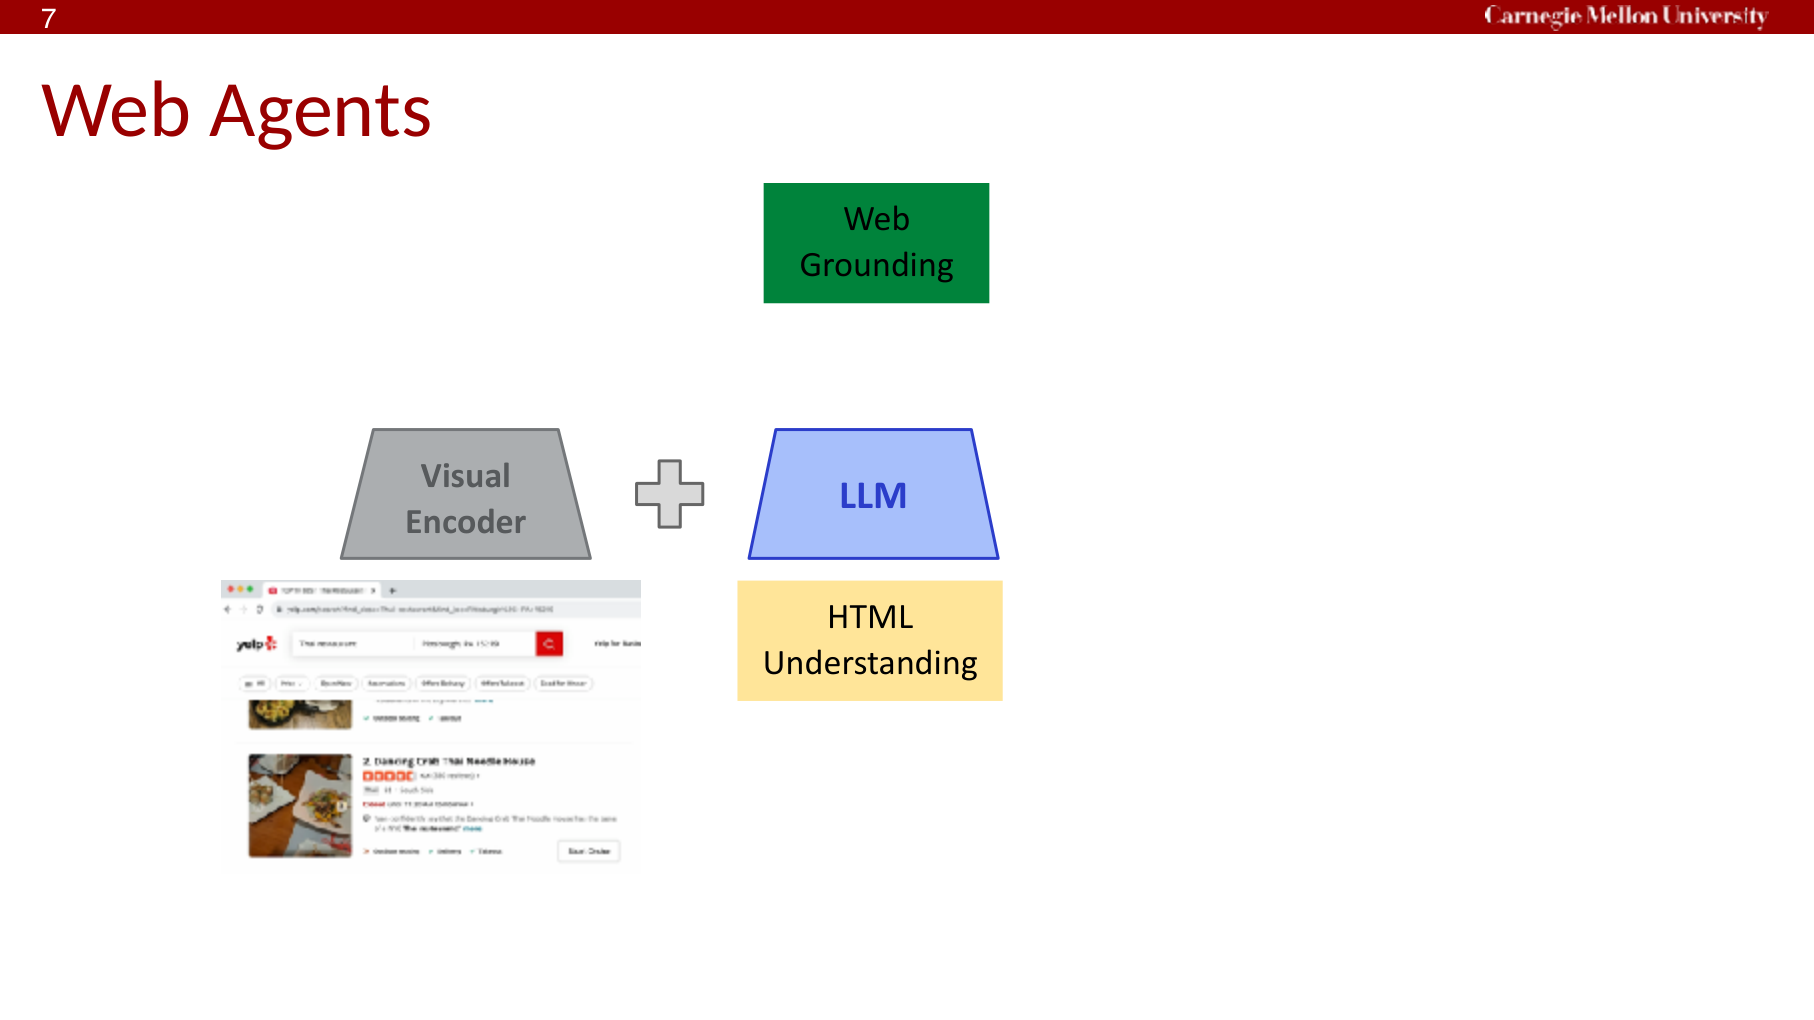
\includegraphics[width=0.82\textwidth]{../lectures/lec06_multimodal_autonomous_agents/figures/lec06_fig_001.png}
\caption{Web agents 的基本栈：视觉、语言、grounding 与网页环境共同决定 agent 的行为。}
\end{figure}

如果任务是“找一个评分最高、评论数超过 200 的泰餐厅”，系统不能只做信息检索。它还要在页面之间跳转、读取视觉元素、区分可点击区域、判断排序结果、避免误操作，并在达到目标后停止。这类问题天然具有三个结构特征：
\begin{itemize}
\item \textbf{部分可观测（partial observability）}：agent 看到的只是当前屏幕和局部 DOM，而不是真实网页状态的完整描述。
\item \textbf{长程交互（long horizon interaction）}：要多步连续做对，不能把任务拆成彼此独立的单跳问答。
\item \textbf{执行正确性（functional correctness）}：很多任务的答案不是一段文本，而是页面状态是否被正确改变、仓库是否被创建、购物流程是否真的完成。
\end{itemize}

这就是为什么本讲会把 \textbf{benchmark realism} 放在第一优先级。没有真实环境，很多 agent 错误根本暴露不出来。

\subsection{为什么纯 HTML 不够：视觉 grounding 是任务语义的一部分}

WebArena 之前的很多方法倾向于把网页转成 HTML、accessibility tree 或压缩后的文本表示，再让 LLM 在文本空间里做决策。这当然有价值，但讲者明确指出 \textbf{HTML is insufficient}。原因不是 HTML 完全没信息，而是现实网页中有大量决定任务成败的内容并不稳定地出现在文本表示里：
\begin{itemize}
\item CSS/JavaScript 动态改变布局与可见状态。
\item 可点击元素的真实位置、层叠关系与视觉显著性不等价于 DOM 顺序。
\item 视觉上下文经常决定“这个按钮是不是用户想要的那个按钮”。
\item 真实任务包含图片比对、商品外观匹配、截图中的表格或地图等视觉约束。
\end{itemize}

这意味着 \textbf{视觉信息并不是附加模态，而是任务语义本身}。当用户说“买这个图里同款但红色的另一个商品”时，文本树再长也不足以替代视觉 grounding。

\begin{knowledgebox}{本讲的核心命题}
对真实 web agents 来说，感知和规划不是两个彼此独立的问题。观测表示一旦失真，后续规划再强也只是在错误状态上做聪明搜索。
\end{knowledgebox}

\section{Benchmark 视角：Mind2Web、WebArena 与 VisualWebArena}

\subsection{三者分别回答什么问题}

这三套资源经常被放在同一条 agent 发展线上，但它们回答的问题并不一样。

\textbf{Mind2Web} 的重点是 \emph{generalist web-agent data}。它收集 137 个真实网站、31 个 domain 上的 2000 多个开放式任务与人工动作序列，目的是让研究者能在真实网站分布上研究泛化。它告诉我们：真实网站远比模拟环境复杂，HTML 也远比玩具环境中的结构化描述更脏、更长、更噪。

\textbf{WebArena} 的重点是 \emph{realistic yet reproducible environment}。它不只给演示数据，而是给出可交互环境、工具站点、知识资源和 execution-based functional checks。也就是说，WebArena 更接近“真实任务环境”，而不是静态轨迹数据集。

\textbf{VisualWebArena} 则继续追问：如果现实网页任务需要图片、布局、界面视觉提示，那么 text-only environment 仍然低估了问题难度。它在 WebArena 的基础上加入 visually grounded tasks 和 visually grounded evaluation，使 benchmark 真正开始衡量多模态网页 agent。

\begin{importantbox}{关键区分}
Mind2Web 偏向 \textbf{离线真实网页数据集}；WebArena 偏向 \textbf{可交互、可复现、execution-based 的文本为主环境}；VisualWebArena 则把同样的 functional evaluation 推向 \textbf{视觉 grounding 必不可少} 的任务空间。
\end{importantbox}

\subsection{VisualWebArena：把视觉放回 functional evaluation}

\begin{figure}[H]
\centering
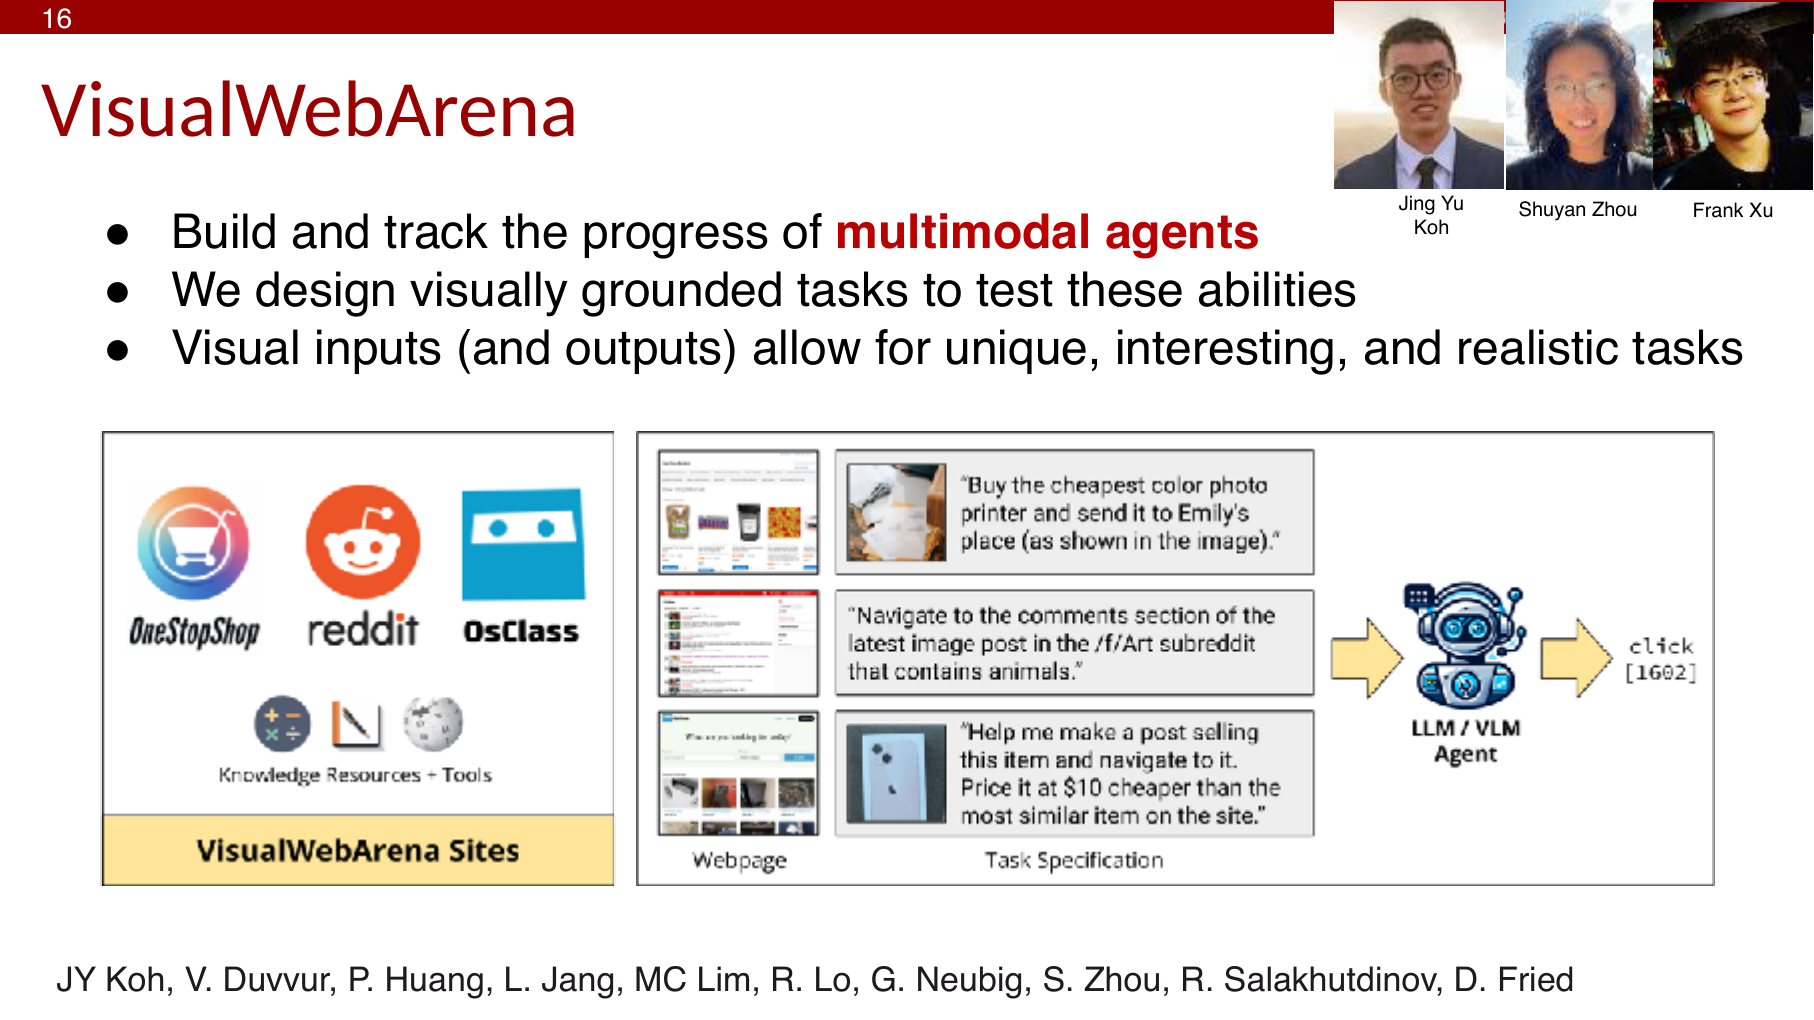
\includegraphics[width=0.82\textwidth]{../lectures/lec06_multimodal_autonomous_agents/figures/lec06_fig_002.png}
\caption{VisualWebArena 的目标是 visually grounded web tasks，而不是只在文本化网页上做导航。}
\end{figure}

讲者用多个任务示例说明 VisualWebArena 为什么必要。比如按图片找到同款商品、在分类广告里比对目标图片、在论坛中根据页面布局进入正确评论区，这些任务都不能靠“读一段 HTML 再回答”来完成。VisualWebArena 的价值在于：
\begin{itemize}
\item 它把 \textbf{视觉-文本联合观测} 变成 benchmark 的默认输入。
\item 它延续 WebArena 的 \textbf{execution-based evaluation}，避免只看文本表面相似度。
\item 它让研究者能定量比较 \textbf{text-based LLM agents} 与 \textbf{multimodal VLM agents} 的差异。
\end{itemize}

从形式上看，这类环境很自然地写成一个 POMDP：
\[
\mathcal{M}=(\mathcal{S},\mathcal{A},\mathcal{O},T,R),\qquad o_t\sim \mathcal{O}(s_t),\ a_t\in\mathcal{A}(o_t).
\]
其中，$\mathcal{S}$ 是网页环境真实状态，$\mathcal{A}$ 是可执行动作集合，$\mathcal{O}$ 决定 agent 在某个状态下能看到的截图、DOM 或 SoM 标记等观测，$T$ 是环境转移，$R$ 则是与 functional correctness 相关的奖励或成功判定。写成这个形式的意义在于：\textbf{agent 的难度不仅在动作选择，也在观测建模。}

\section{从 VLM Agents 到 Inference-Time Search}

\subsection{SoM、规划与 failure modes}

讲者随后转向 \textbf{Visual Language Models as Agents}。slides 强调的不是“换一个更大的 VLM 就好”，而是要给模型一种更适合交互界面的表示。Set-of-Marks（SoM）风格的表示就是代表例子：把可交互元素显式标记出来，帮助模型在图像空间中定位 candidate actions。

\begin{figure}[H]
\centering
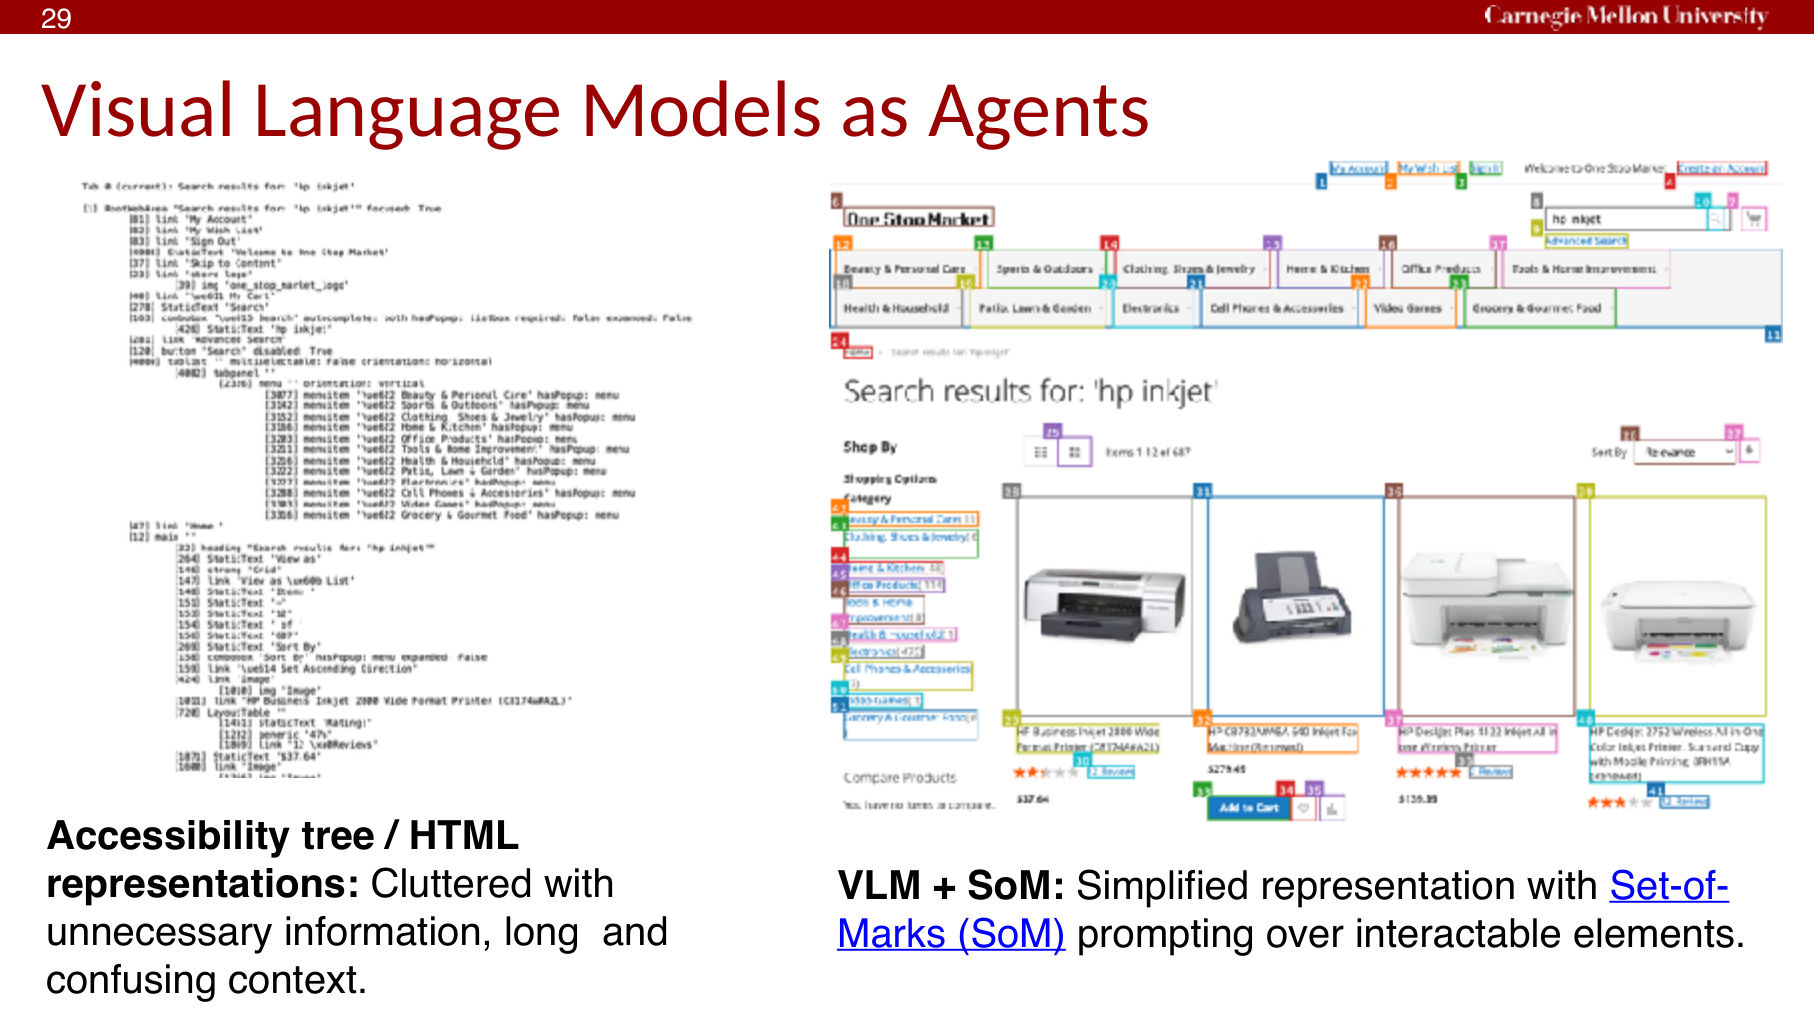
\includegraphics[width=0.72\textwidth]{../lectures/lec06_multimodal_autonomous_agents/figures/lec06_fig_003.png}
\caption{SoM 风格表示把交互元素变成更明确的视觉候选，缓解 cluttered interfaces 带来的歧义。}
\end{figure}

同时，web agent 还需要一个更完整的系统架构：
\begin{figure}[H]
\centering
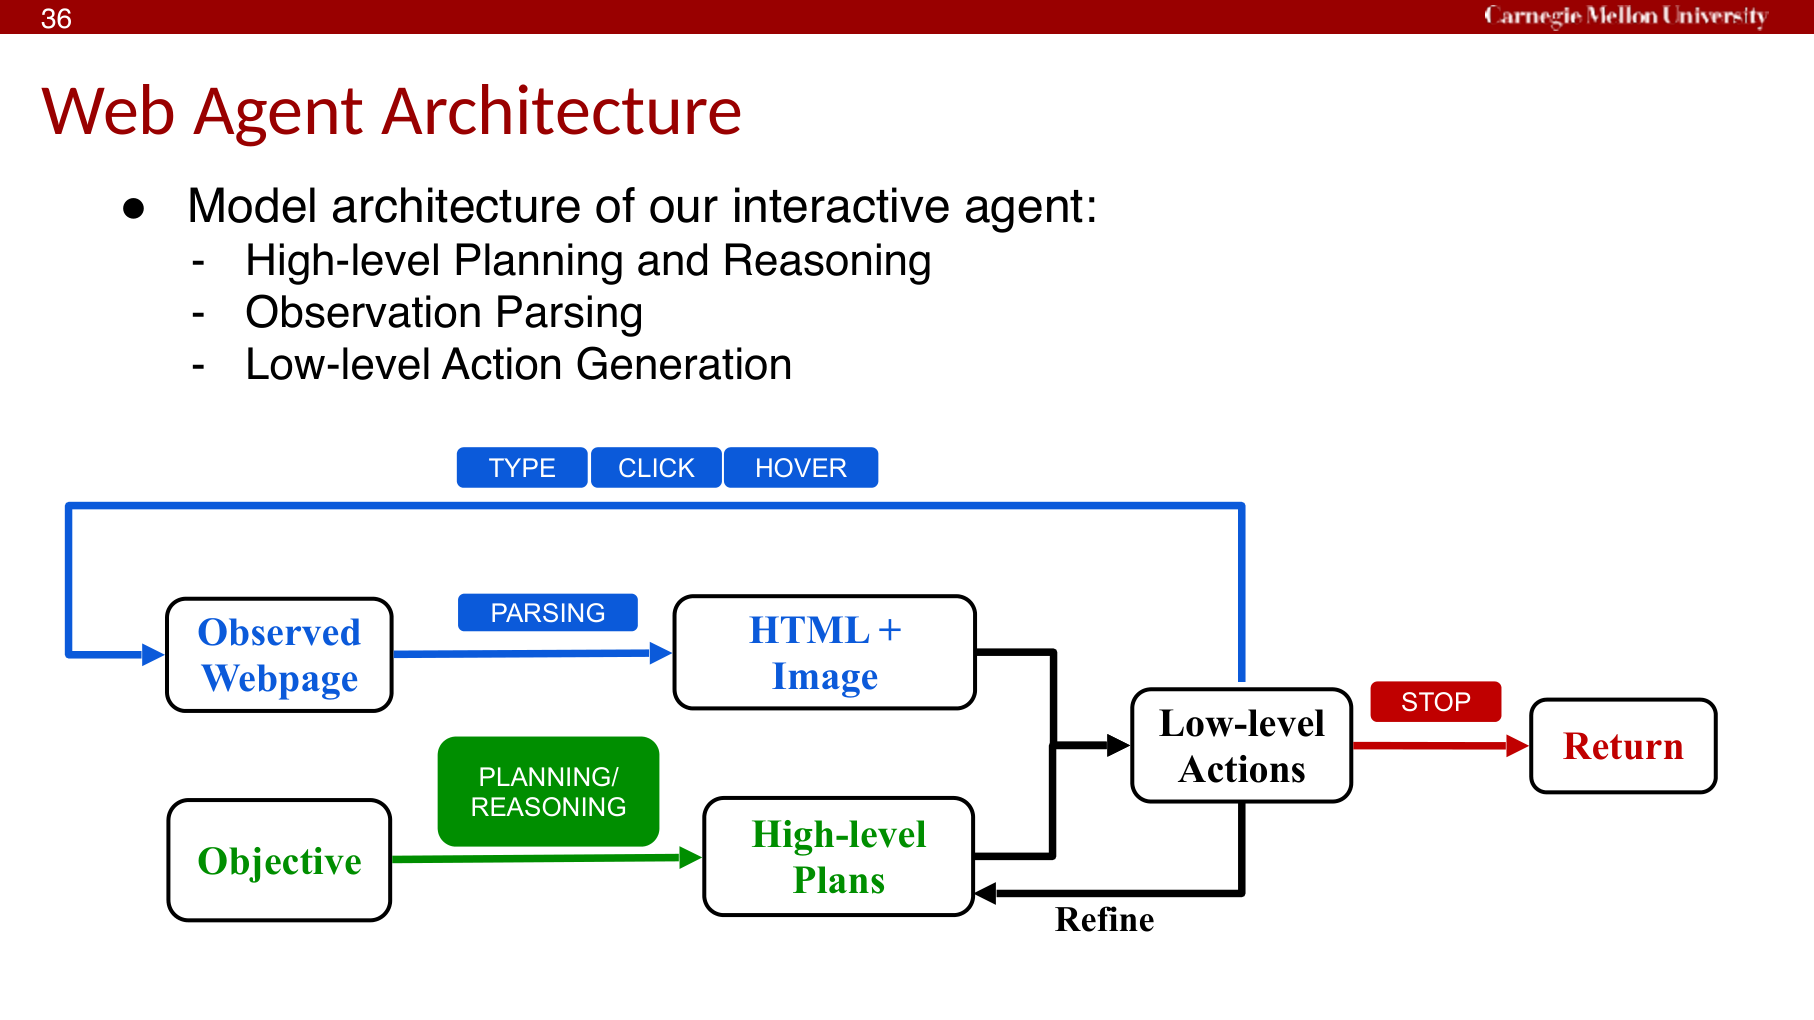
\includegraphics[width=0.80\textwidth]{../lectures/lec06_multimodal_autonomous_agents/figures/lec06_fig_004.png}
\caption{Web agent architecture 需要同时处理观测、低层动作、计划状态与环境反馈。}
\end{figure}

这里有一个关键认识：\textbf{低层动作正确，并不代表全局任务正确。} 例如某一步点击看起来合理，但会把 agent 带进错误页面；又例如 agent 一度完成了正确操作，随后又因为没有保持全局目标状态而把它撤销。这些 failure modes 在 slides 中被明确列出，包括在页面间来回 oscillate、卡在 loop 里、或者做对一部分又在后续步骤 undo 掉。

\subsection{为什么长程任务会出现 error compounding}

\begin{figure}[H]
\centering
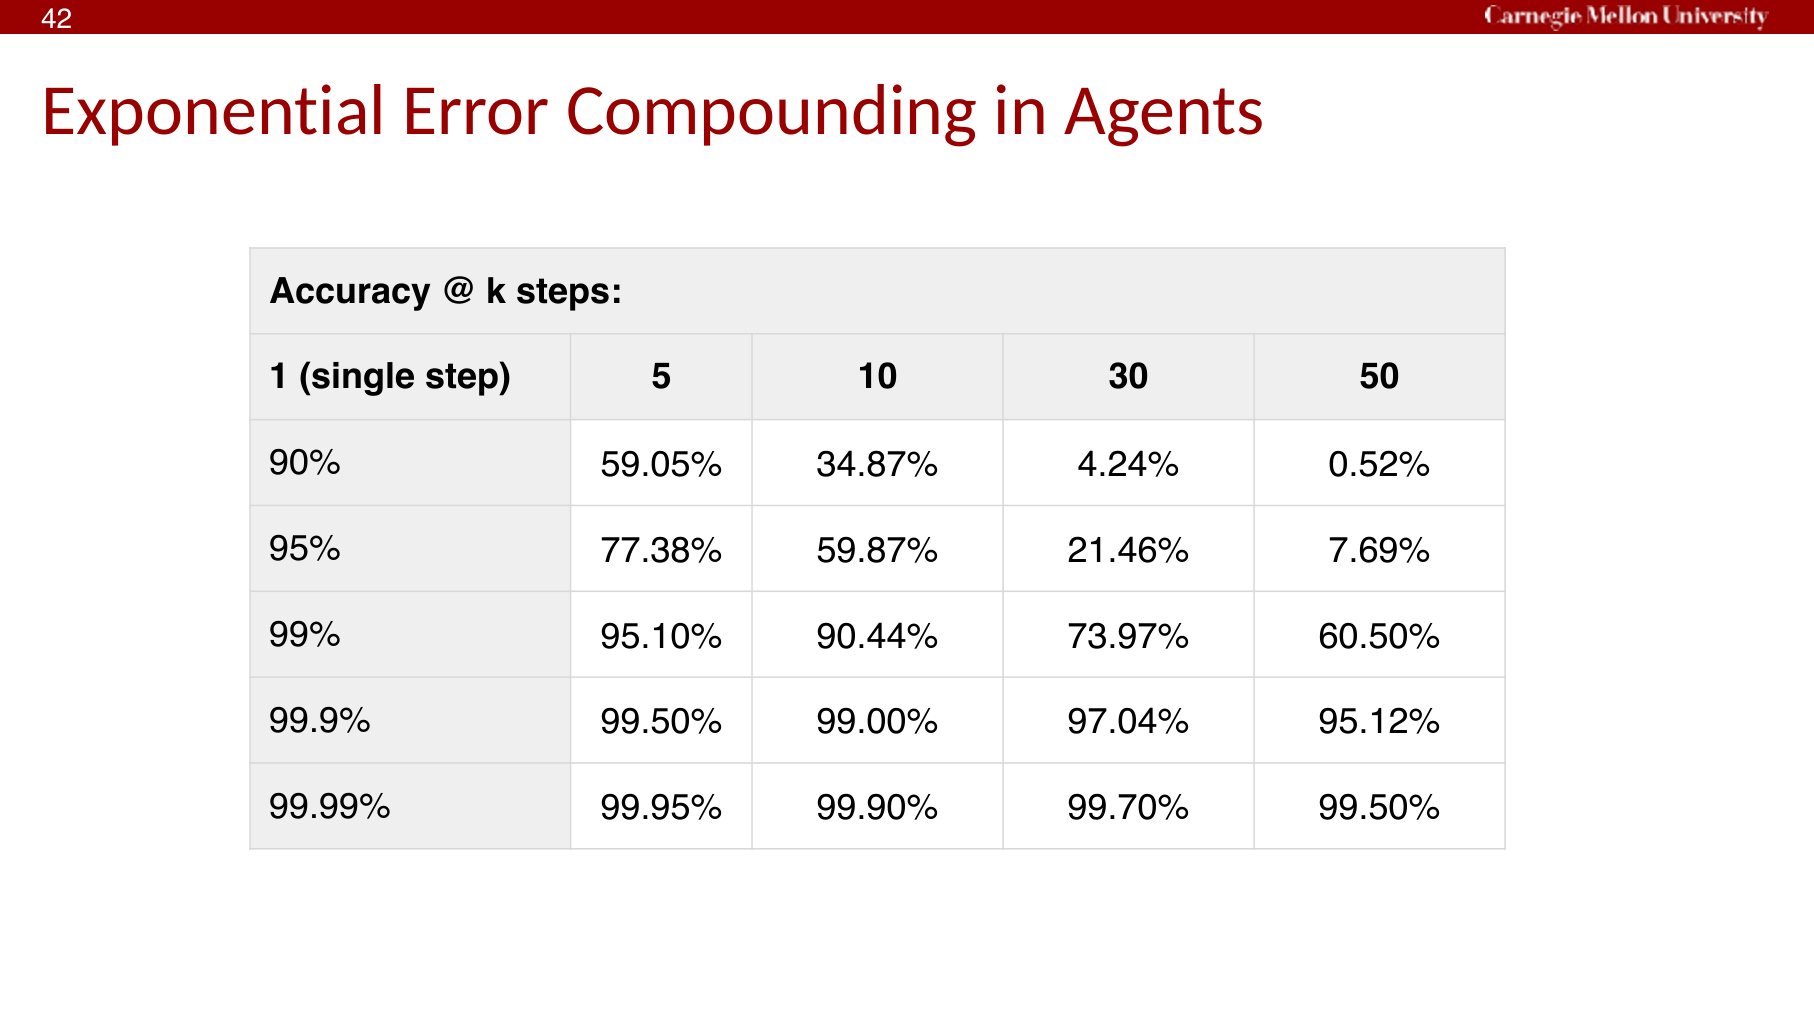
\includegraphics[width=0.74\textwidth]{../lectures/lec06_multimodal_autonomous_agents/figures/lec06_fig_005.png}
\caption{长程任务中的误差累积：即使单步准确率尚可，整条 trajectory 的成功率也会快速下降。}
\end{figure}

这一页最值得教材化展开的地方在于，讲者并不是在说“模型还不够强”，而是在说 \textbf{autonomous agents 的误差结构和单轮问答完全不同}。如果把每一步大致视作正确率为 $p$ 的决策，那么长程任务近似成功率会像
\[
\Pr(\text{success at }k\text{ steps}) \approx p^k
\]
那样快速下降。这里 $p$ 是近似单步正确率，$k$ 是必须连续做对的交互步数。这个公式并不追求严格统计精确，而是帮助读者抓住本讲的核心直觉：\textbf{local decisions have global consequences}。

因此，单纯 repeated sampling 并不能根治问题。你可以多采几条完整 trajectory，但搜索空间是指数大的，而且如果没有对 \emph{中间状态} 的判断能力，系统很难知道什么时候该继续扩展、什么时候该 backtrack。

\subsection{Tree Search for Language Model Agents}

\begin{figure}[H]
\centering
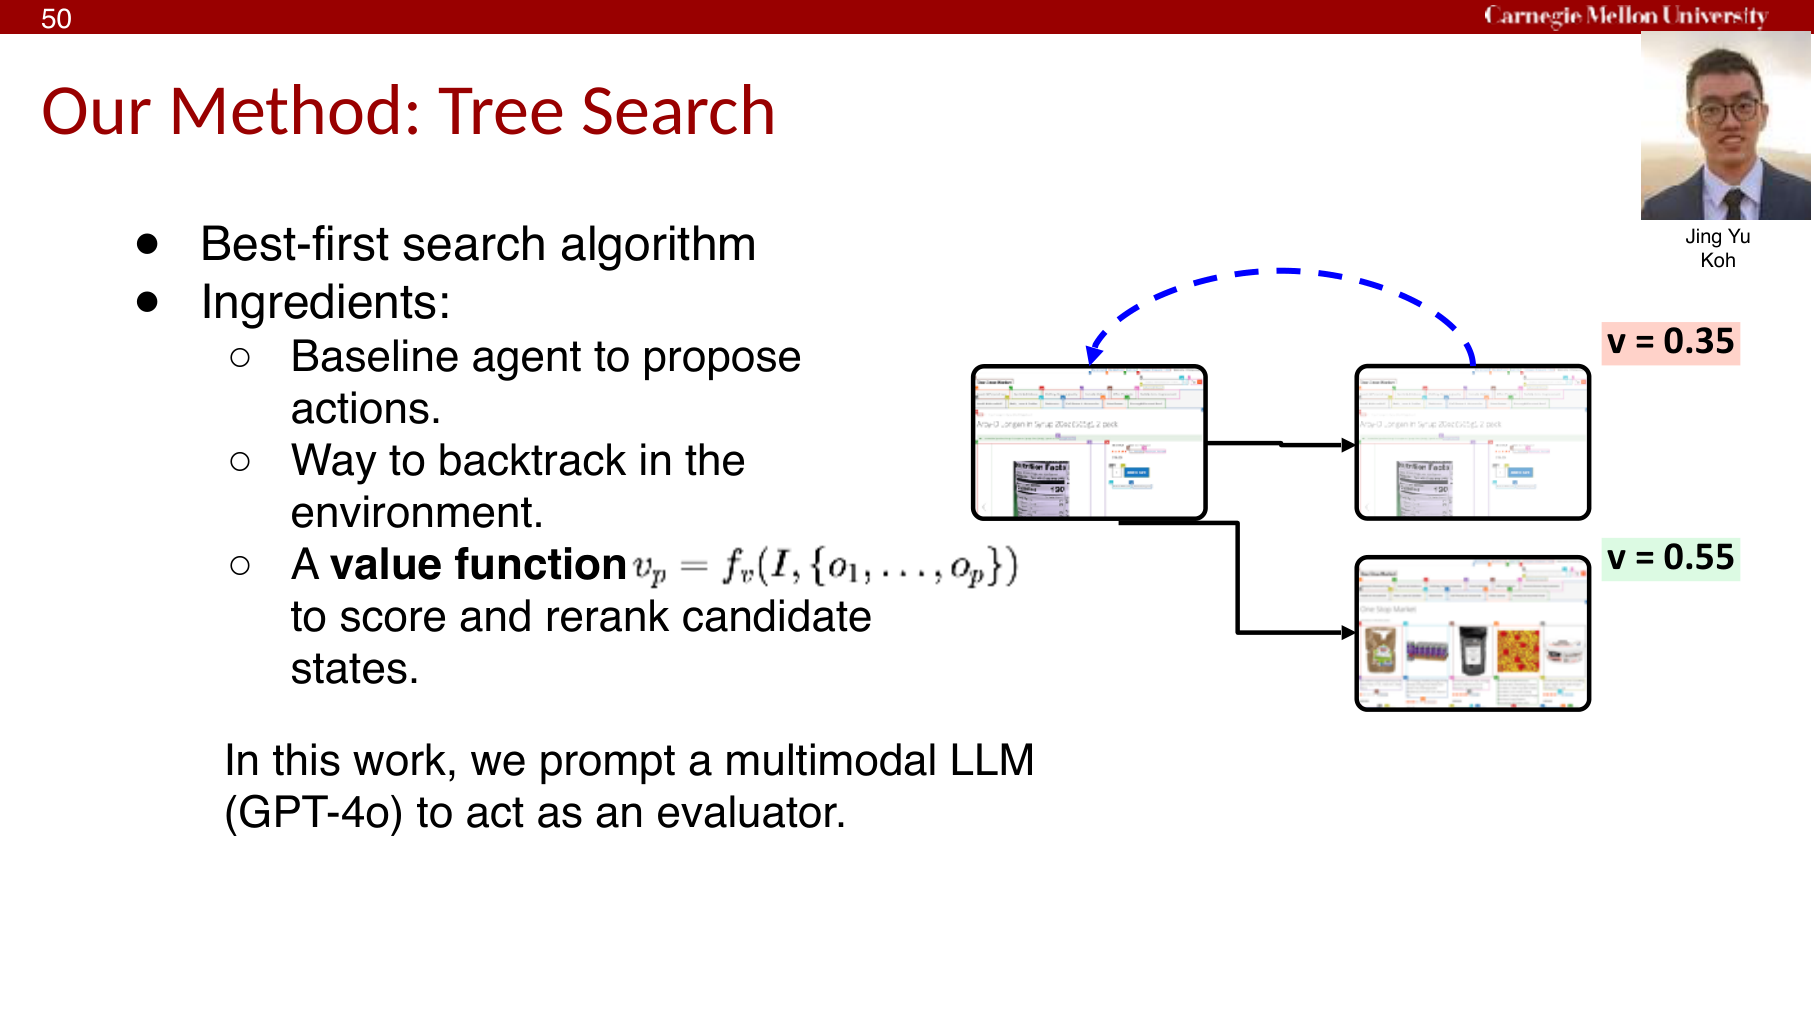
\includegraphics[width=0.76\textwidth]{../lectures/lec06_multimodal_autonomous_agents/figures/lec06_fig_006.png}
\caption{Tree Search 的核心 ingredients：baseline policy 负责提议分支，value function 负责评估中间状态。}
\end{figure}

这正是 \textbf{Tree Search for Language Model Agents} 的出发点。它的基本想法是：不要把 agent 当成只能沿一条 trajectory 前进的策略，而要把它当成一个能提出候选 action branches 的 proposal model；然后再配一个 \textbf{value function} 去评估中间状态的潜力。一个简化写法是：
\[
\hat{s}_t = \arg\max_{s \in \mathcal{F}_t} v_\phi(s),\qquad \mathcal{F}_{t+1}=\operatorname{Expand}(\hat{s}_t; b,d,c).
\]
这里 $\mathcal{F}_t$ 是当前 frontier，$v_\phi(s)$ 是中间状态评分函数，$b,d,c$ 分别控制 branching factor、search depth 与总 budget。直觉上，它做的是“在有限预算下，优先把算力用在最有希望的 partial trajectories 上”。

\begin{lstlisting}
initialize frontier with current state
while budget remains:
    pop highest-value state
    if value exceeds threshold: commit
    expand candidate actions from baseline agent
    evaluate children with value function
return best state found
\end{lstlisting}

这个算法与 L01 中讲到的 test-time search 形成了直接呼应。区别在于，这里 search 的对象不是思维链节点，而是 \textbf{真实环境中的交互状态}。因此它不仅要考虑 reasoning quality，还要考虑页面回退、环境恢复和 backtracking 成本。

\subsection{实验结论、compute tradeoff 与局限性}

\begin{figure}[H]
\centering
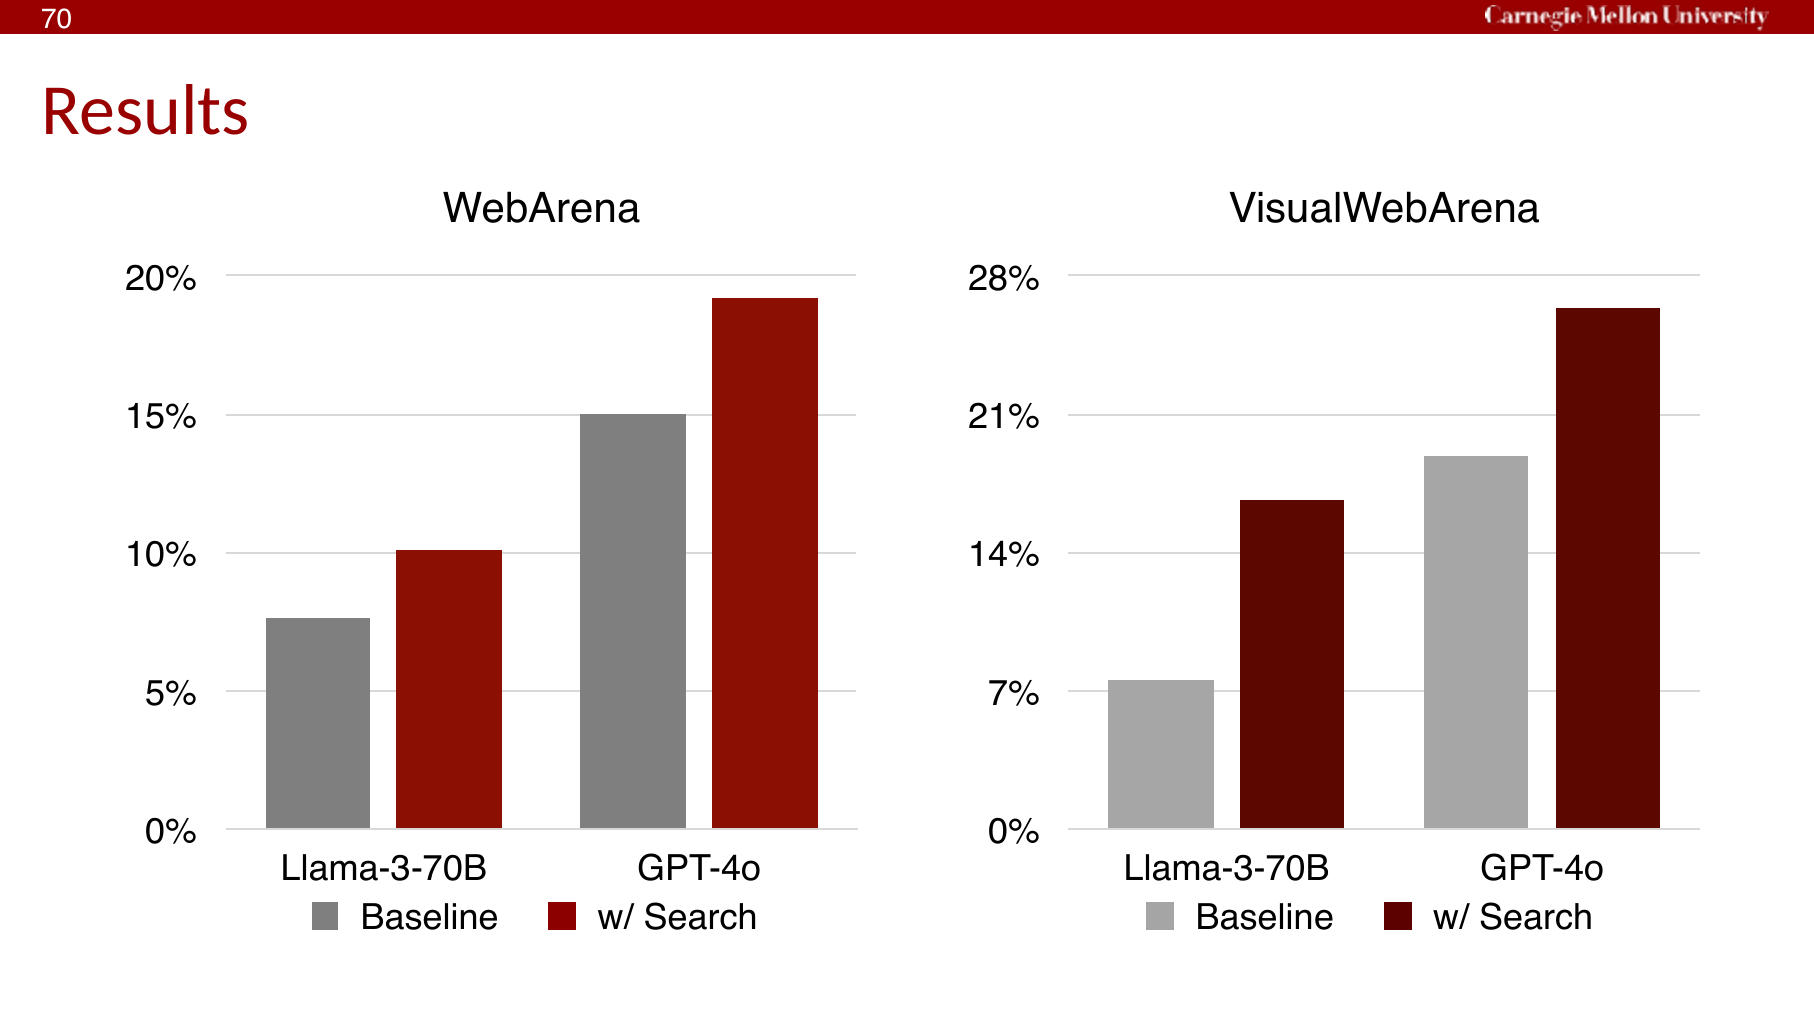
\includegraphics[width=0.76\textwidth]{../lectures/lec06_multimodal_autonomous_agents/figures/lec06_fig_007.png}
\caption{Search 可以显著提高 success rate，但与 human performance 仍有巨大差距。}
\end{figure}

讲者给出的结果很重要，因为它同时包含 \textbf{正面结论} 和 \textbf{系统局限}。

正面结论是：在 VisualWebArena 和 WebArena 上，把 search 加到 baseline GPT-4o agent 上，成功率会有显著提升。项目页也明确指出，VisualWebArena 上相对提升接近 40\%，并且随着 search budget 增加，表现一般会继续上升。这说明 \textbf{inference-time compute 在 realistic web agents 上是真正有效的设计变量}。

局限性同样清楚：
\begin{itemize}
\item search 很慢，因为回溯到旧状态在现实网页环境中代价高。
\item 结果高度依赖 value function 质量；若 value model 不会判断中间状态是否有前景，search 只会更昂贵地走错路。
\item baseline policy 太弱时，frontier 里本来就没有好分支，search 的上限也会受限。
\end{itemize}

因此，讲者后来把当前工作概括为三条方向：把 search 当成 policy improvement operator、微调更强的 value function、并系统研究 baseline agent 与 search budget 的 compute tradeoff。这一点与 L01 的 reasoning-time scaling 视角完全一致。

\section{Agents Suffer From A Data Problem}

\subsection{为什么 agent training 特别缺数据}

本讲中最值得注意的一句判断是：\textbf{agents suffer from a data problem}。原因很直接。LLM 可以从大规模现成文本中预训练，但 GUI 或 web agents 所需的不是普通文本，而是带有环境状态、操作步骤和完成判定的 trajectory data。人工标注这种数据非常贵，而且可扩展性极差。

这意味着很多今天的 agent 实践其实是：\textbf{先离线训练一个模型，再在几乎没有针对性 agent 经验的数据分布上 zero-shot 部署。} 这样做当然能跑出 demo，但遇到真实 benchmark 时很快会暴露出规划、state tracking 和 grounding 的不足。

\subsection{InSTA：用 synthetic tasks 扩大训练分布}

讲者随后介绍 \textbf{Towards Internet-Scale Training For Agents (InSTA)}。其目标不是凭空“合成一点数据”，而是把互联网本身变成 task source，再用模型生成、筛选、验证 agentic tasks，从而把训练分布扩展到更大范围的网站。

\begin{figure}[H]
\centering
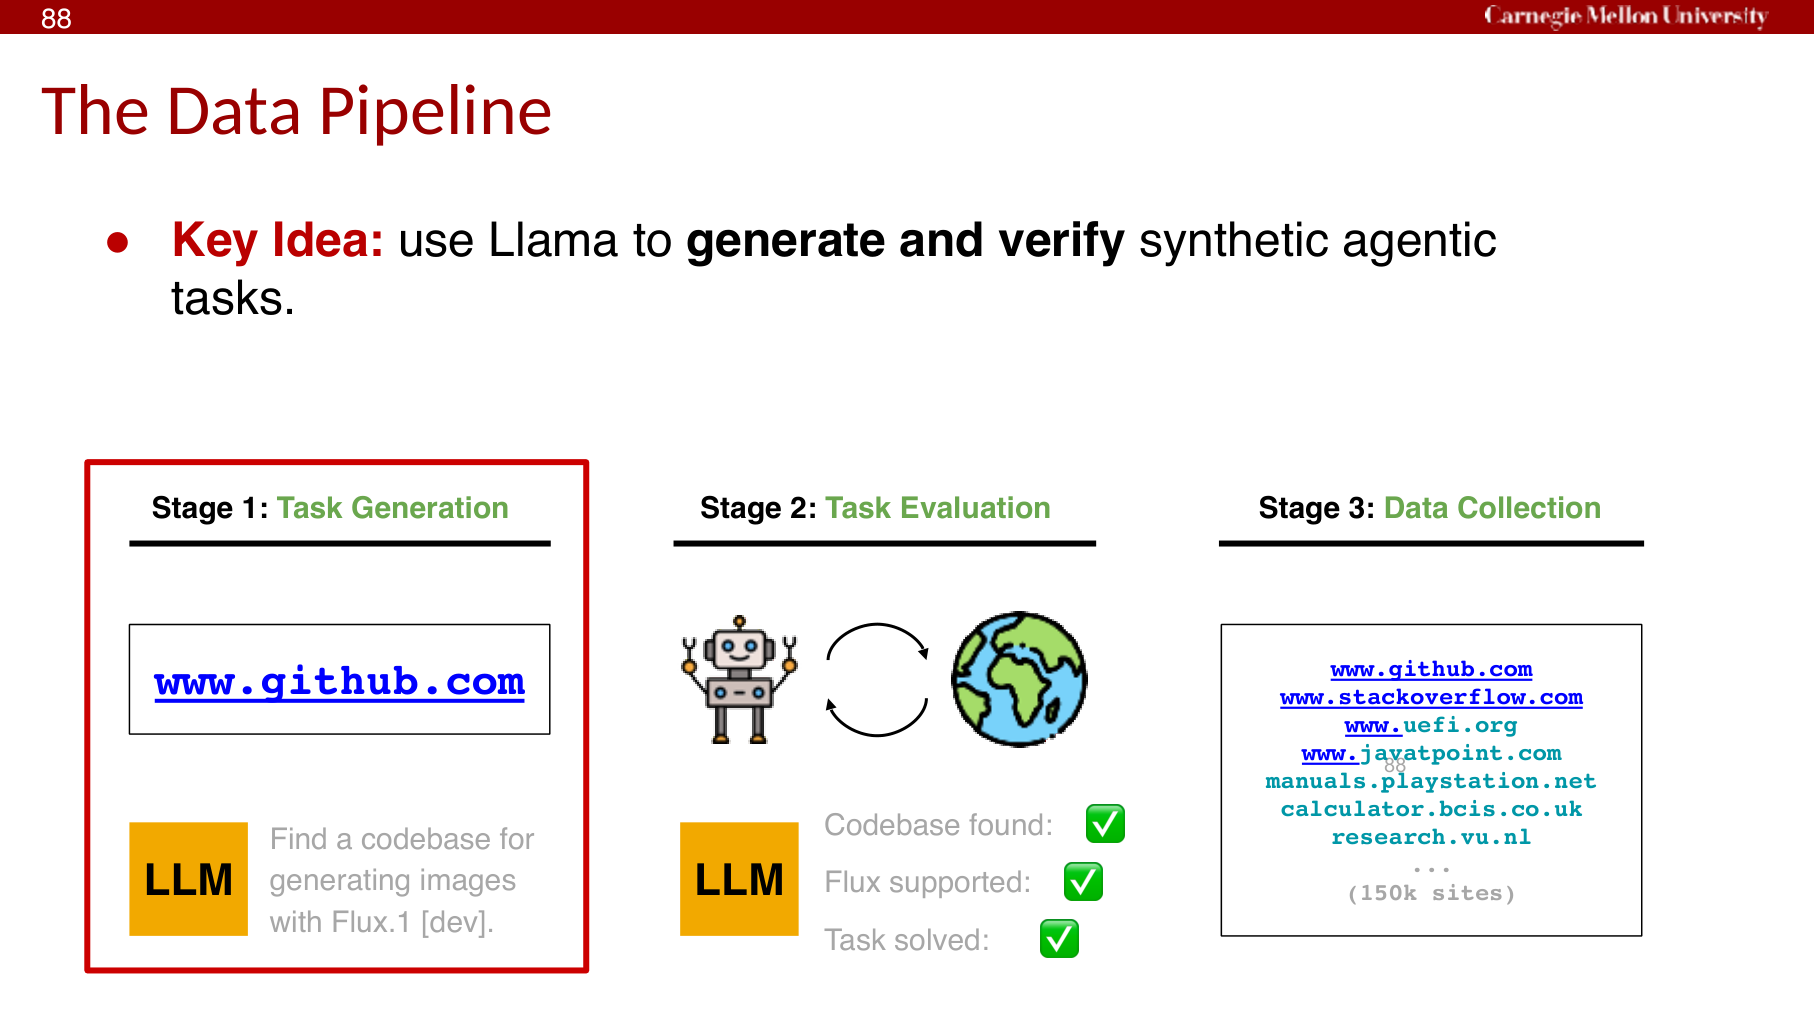
\includegraphics[width=0.78\textwidth]{../lectures/lec06_multimodal_autonomous_agents/figures/lec06_fig_008.png}
\caption{InSTA 的管线：从 web domains 生成 realistic tasks，再做验证与扩展。}
\end{figure}

其基本循环可以写成：
\begin{lstlisting}
sample a web domain
use Llama to propose realistic tasks
run/inspect trajectories
estimate task success with verifier
keep feasible and solvable tasks for large-scale training
\end{lstlisting}

这一步与静态 instruction generation 的区别在于，生成出来的任务要能 \textbf{被 agent 真正在环境中执行和验证}。也就是说，task generation 必须与 task verification 配对。

\begin{figure}[H]
\centering
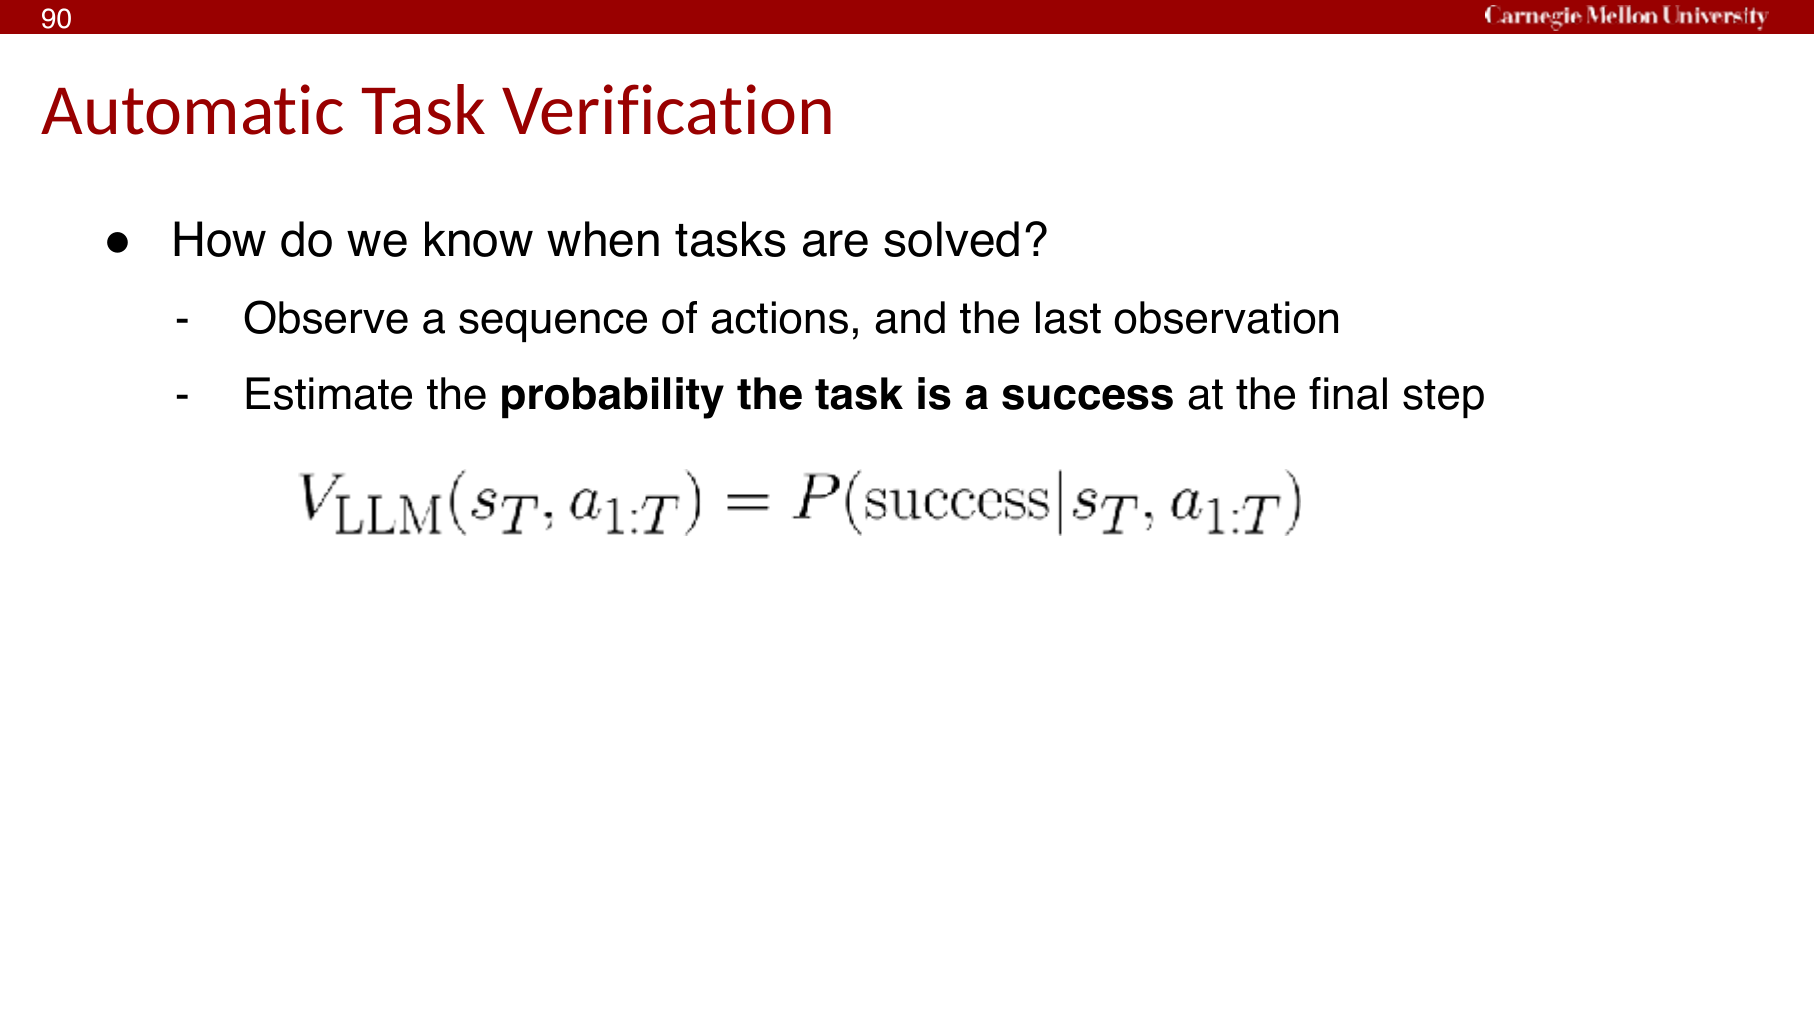
\includegraphics[width=0.78\textwidth]{../lectures/lec06_multimodal_autonomous_agents/figures/lec06_fig_009.png}
\caption{Automatic task verification：观察轨迹与最终状态，估计任务是否真正成功。}
\end{figure}

教材化看，这里的核心不是某个具体 Llama prompt，而是：\textbf{agent data pipeline 必须同时回答“任务是什么”“怎么知道做成了”“怎么扩大规模”三个问题。} 如果只会生成 instruction，而不会验证任务完成，那么最终只是在制造噪声 supervision。

\begin{warningbox}{为什么 synthetic data 不是万能药}
Synthetic tasks 可以扩展覆盖面，但并不会自动保证 realism、safety 或 distribution match。生成出来的任务也可能偏向信息检索、回避状态修改、或隐含不安全网站。lecture slides 提到的 filtering 和 feasibility checks，正是在防止这种漂移。
\end{warningbox}

\section{从 Web Agents 到 Physical Agents}

\subsection{Perception-action loop 在机器人里更严苛}

讲者最后把视角从网页转向 physical agents。这个转向很重要，因为它说明本讲不是一组离散 case studies，而是在强调一种更一般的 multimodal autonomy 框架：\textbf{感知、规划、状态估计、动作执行与反馈修正的闭环。}

\begin{figure}[H]
\centering
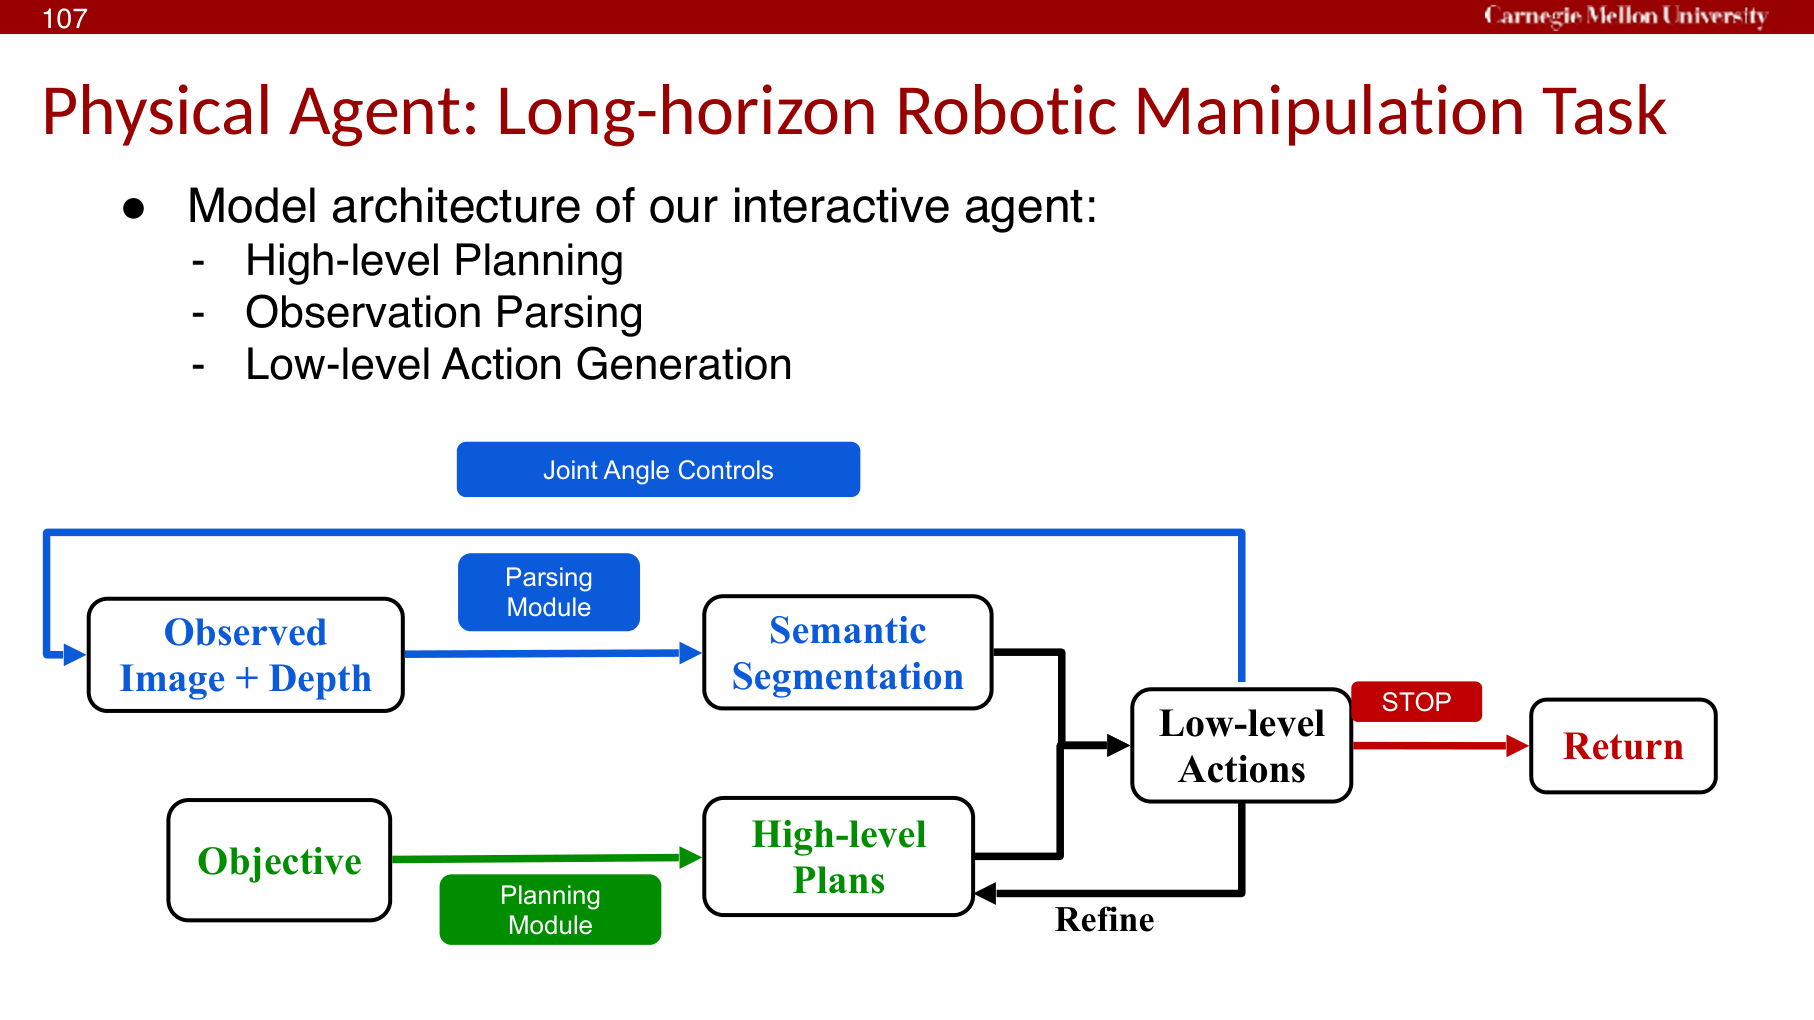
\includegraphics[width=0.80\textwidth]{../lectures/lec06_multimodal_autonomous_agents/figures/lec06_fig_010.png}
\caption{Physical agent 的输入包括 image、depth 和 semantic segmentation，因而比 web agent 更接近 embodied autonomy。}
\end{figure}

与 web agents 相比，physical agents 至少多了三层难度：
\begin{itemize}
\item 视觉误差会直接传导到物理执行误差。
\item 环境状态恢复成本更高，错误动作代价更大。
\item 成功往往要依赖多个连续子任务都完成，因此长程成功率更加脆弱。
\end{itemize}

\subsection{Plan-Seq-Learn：分层解决 long-horizon manipulation}

\begin{figure}[H]
\centering
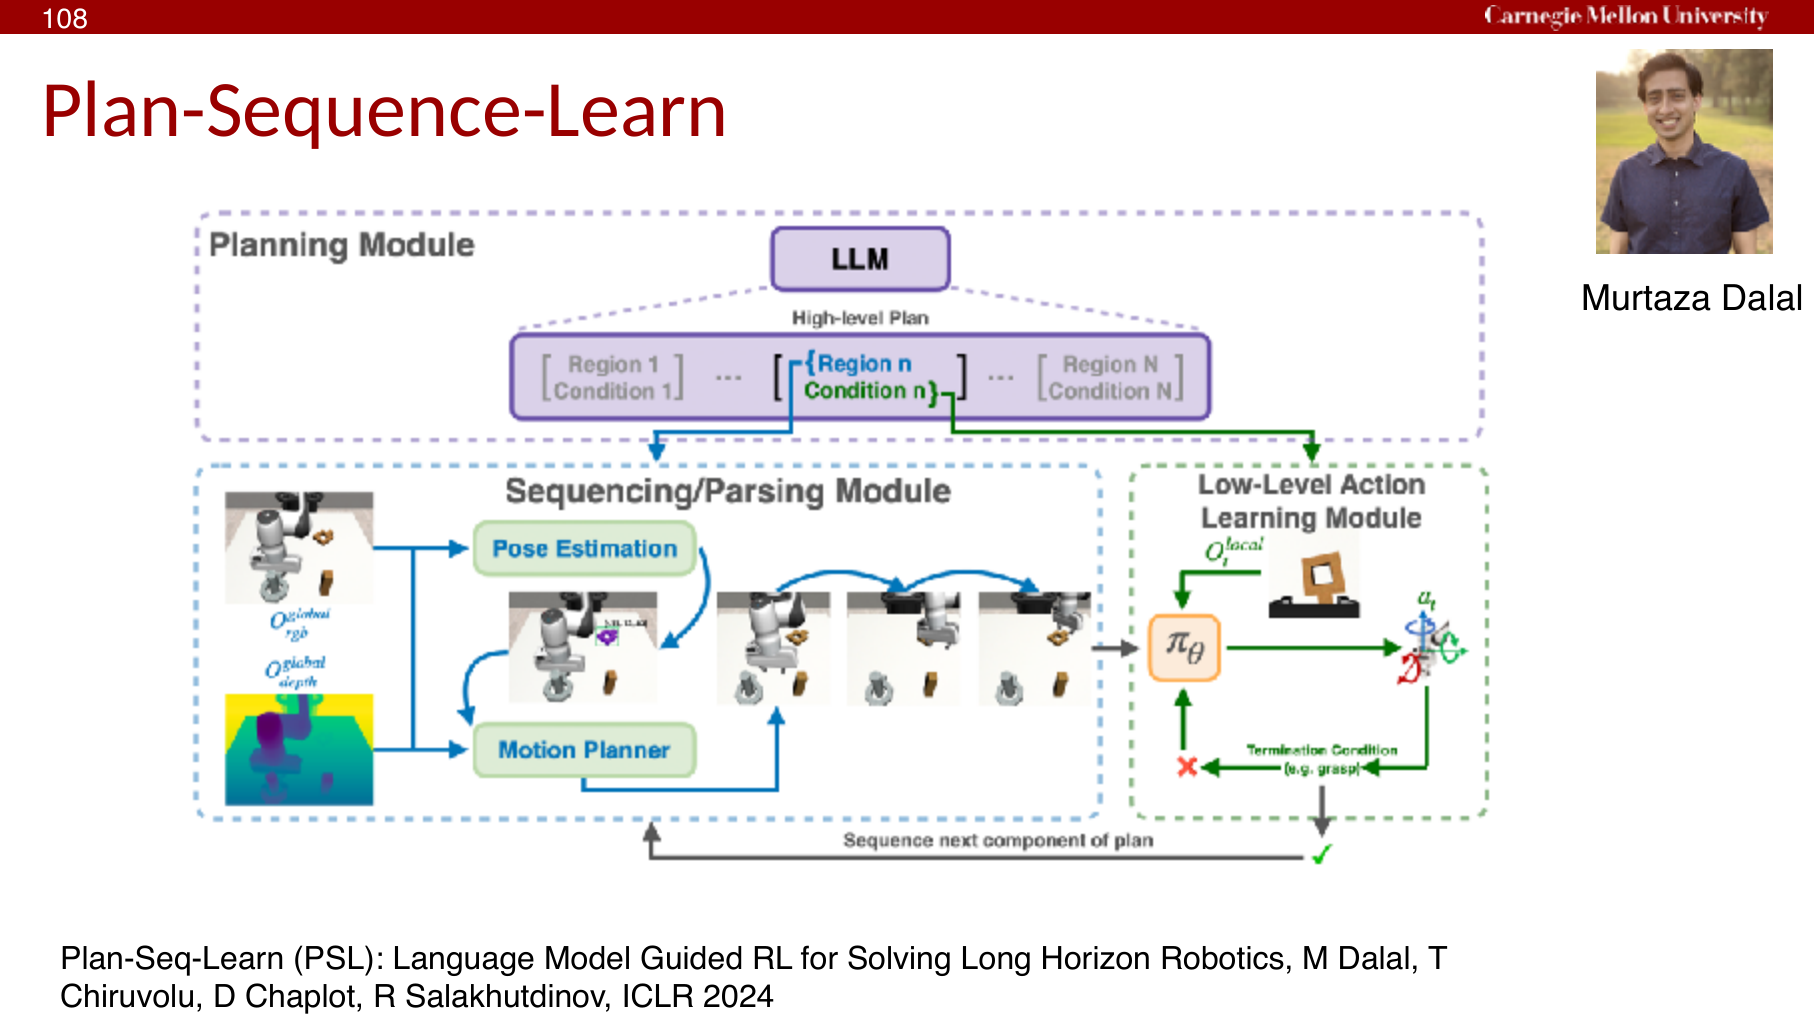
\includegraphics[width=0.82\textwidth]{../lectures/lec06_multimodal_autonomous_agents/figures/lec06_fig_011.png}
\caption{Plan-Seq-Learn 用语言规划、scene grounding 和局部 RL control 分层处理 manipulation。}
\end{figure}

Plan-Seq-Learn 的核心不是把一个大模型直接端到端映射到所有控制信号，而是先把任务拆成可管理的层级。slides 明确给出 manipulation 成功率可写成：
\[
P(\mathrm{success}) = P(\mathrm{task}_1) \cdot P(\mathrm{task}_2\mid \mathrm{task}_1) \cdots P(\mathrm{task}_n\mid \mathrm{task}_{<n}).
\]
其中每个 $\mathrm{task}_i$ 是一个子目标或阶段。这个公式的直觉与 error compounding 完全一致：如果每一步都只有中等成功率，那么整体 success 会迅速坍缩。因此系统必须：
\begin{itemize}
\item 用 \textbf{language planner} 生成结构化的高层子目标。
\item 用 \textbf{sequencing / parsing module} 把语言子目标对齐到当前场景中的对象与条件。
\item 用 \textbf{local RL controller} 学习低层 interaction policies，而不是为每个阶段单独写控制器。
\end{itemize}

\begin{lstlisting}
language planner proposes structured subgoals
sequencing module grounds each subgoal in the scene
local RL controller executes low-level actions
feedback updates the next subgoal execution
\end{lstlisting}

这种设计的意义在于：它把高层 reasoning、环境 grounding 和 motor control 分开，使每层都能利用更合适的 inductive bias。它也揭示出与 GUI agents 的共性：\textbf{不是所有多模态 agent 都应该追求一个“单模型一步到位”的方案。}

\section{Readings 与跨讲联系}

本讲的 readings 形成一条清晰链条。\textbf{Mind2Web} 说明真实网站数据的分布与离线行为建模难题；\textbf{WebArena} 把问题升级为可交互、可复现、execution-based 的现实环境；\textbf{VisualWebArena} 证明视觉 grounding 必须进入 benchmark；\textbf{Tree Search for Language Model Agents} 则说明 inference-time compute 可以直接改变 realistic web tasks 上的 success rate。

与 L01 的关系尤其直接。L01 主要讨论在 reasoning task 上如何把 test-time compute 分配给更长、更宽、更可验证的 search 过程；本讲则把同样的思想搬到了 \textbf{真实环境中的 multimodal agents}：候选不再只是 reasoning trace，而是环境状态与动作序列。下一讲如果继续推进 GUI/OS agents，这里的 benchmark distinction、grounding 问题与 data bottleneck 都会成为前提。

\section{本章小结}

\begin{figure}[H]
\centering
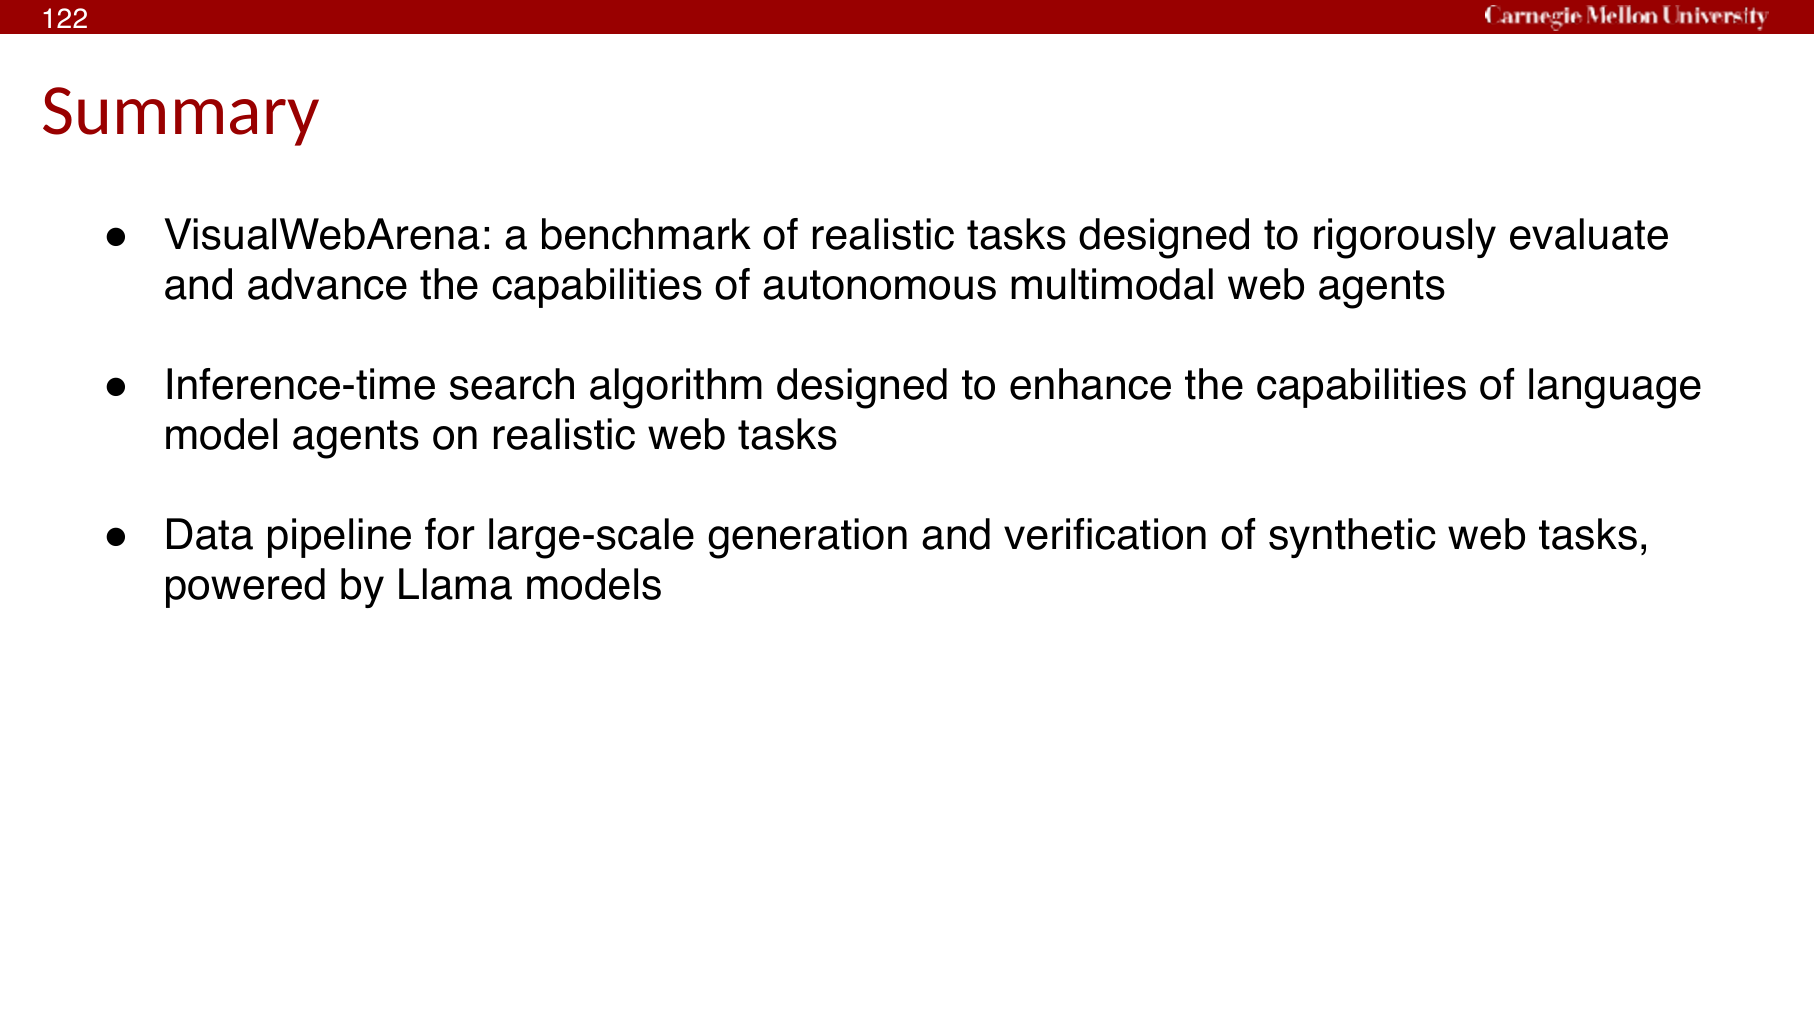
\includegraphics[width=0.80\textwidth]{../lectures/lec06_multimodal_autonomous_agents/figures/lec06_fig_012.png}
\caption{本讲最终把 benchmark、search、synthetic data 和 robotics 串成一条多模态 autonomy 主线。}
\end{figure}

本讲最重要的结论可以压缩成四句：
\begin{enumerate}
\item 对真实 web agents 来说，\textbf{benchmark realism} 是第一性问题；没有 environment，很多错误无法被 functional correctness 揭示。
\item 视觉 grounding 不是“加一点图像输入”，而是网页任务语义本身的一部分，因此 \textbf{VisualWebArena} 这类 benchmark 不可替代。
\item \textbf{Tree search} 证明 inference-time compute 对 multimodal agents 同样有效，但它高度依赖 value function 质量和系统预算。
\item 无论是 web agents 还是 physical agents，最终都绕不开 \textbf{data pipeline、grounding quality、long-horizon planning} 三个系统瓶颈。
\end{enumerate}

\section{复习题}
\begin{enumerate}
\item 用自己的话区分 Mind2Web、WebArena 和 VisualWebArena 的主要目标。
\item 为什么讲者说 HTML-only representation 对真实网页任务不够？
\item Tree search 为什么需要 value function，而不是只做 repeated sampling？
\item InSTA 的 automatic verification 在数据管线里起什么作用？
\item 为什么 physical agents 比 web agents 更强调 perception-action loop 的稳定性？
\end{enumerate}

\section{深入思考题}
\begin{enumerate}
\item 如果你只能改进 baseline agent、value function、search budget 三者之一，你会优先改哪个？为什么？
\item 对网页 agent 来说，视觉 grounding 与长程规划哪个是更基础的瓶颈？请给出任务依赖的回答。
\item Plan-Seq-Learn 这种分层结构是否会限制端到端性能上限？在什么情况下它反而是必要的？
\end{enumerate}

\section{延伸阅读}
\begin{itemize}
\item Mind2Web: Towards a Generalist Agent for the Web.
\item WebArena: A Realistic Web Environment for Building Autonomous Agents.
\item VisualWebArena: Evaluating Multimodal Agents on Realistic Visual Web Tasks.
\item Tree Search for Language Model Agents.
\item Plan-Seq-Learn: Language Model Guided RL for Long-Horizon Robotics.
\end{itemize}
